\documentclass[conference]{IEEEtran}
\usepackage{amsmath,amssymb,mathtools}
\usepackage{graphicx}
\usepackage{tikz}
\usetikzlibrary{arrows.meta,positioning,shapes.geometric,calc}
\usepackage{booktabs}
\usepackage{url}
\usepackage{cite}
\usepackage{caption}
\captionsetup{font=small}

\begin{document}

\title{Predictive Tracking and Elevation Pointing Control\\ for a Maneuvering Object}

\author{\IEEEauthorblockN{Ishaan Mondal}
\IEEEauthorblockA{Department of Mechanical Engineering\\ Indian Institute of Technology Bombay\\ ishaanmondal2005@gmail.com}}

\maketitle

\begin{abstract}
We design and evaluate a predictive-feedback control system for the elevation axis of a single-axis pointing mount tracking a maneuvering object from noisy polar (range, line-of-sight angle) measurements at 20~Hz. The architecture couples a constant-acceleration Kalman filter in Cartesian coordinates, a fixed 0.5~s prediction horizon, and a single low-bandwidth lag compensator designed from a first-principles electromechanical plant model. The compensator's pole is chosen so that its closed-loop lag exactly matches the prediction horizon, removing the dominant source of pointing error without retuning across scenarios. One finalized design, never retuned, is evaluated on the three standardized scenarios and on 40 randomized bounded maneuvers with randomized sensor-loss intervals, achieving 100\% interception success with a mean post-acquisition RMS miss distance of 0.98~m and a mean first-hit time of 2.87~s.
\end{abstract}

\section{Introduction}
Predictive pointing control --- estimating a target's motion from noisy sensor returns and aiming a mount ahead of its current position to compensate for aiming-loop lag --- is a classical problem in electromechanical fire control, exemplified historically by the Kerrison Predictor and the Bell Labs M9 director. Its modern form is identical in structure to antenna tracking, telescope pointing, camera-gimbal stabilization, and drone-landing guidance: a noisy sensor, a state estimator, a short-horizon kinematic predictor, and a conventional feedback loop driving a physical actuator with finite bandwidth and saturation limits. This paper treats the problem in that modern form, purely as an estimation, prediction, and linear-feedback-control exercise; no physical hardware is built.

\textbf{Objective.} Design one fixed estimator/predictor/controller triple for the elevation axis of a mount described in Sec.~\ref{sec:plant}, that (i) estimates a 2-D Cartesian target state from noisy range/angle measurements, (ii) predicts the state 0.5~s ahead, (iii) converts the prediction to an elevation reference, (iv) drives the mount with a single LTI compensator respecting voltage and angle limits, and (v) issues discrete pointing pulses with a 1~s refractory period, without retuning between scenarios or evaluation cases.

\textbf{Assumptions.} Target motion is smooth and bounded ($800$--$2000$~m range, $\le150$~m/s speed, $\le20$~m/s$^2$ acceleration); the sensor is co-located with the mount and may drop out for up to 0.5~s; the mount is rigid with a single dominant structural mode.

\textbf{Approach summary.} We use a constant-acceleration (CA) discrete Kalman filter in Cartesian coordinates (Sec.~\ref{sec:est}) feeding a fixed 0.5~s kinematic prediction, and a single first-order lag compensator $G_c(s)=K_p/(1+s/p)$ (Sec.~\ref{sec:ctrl}) whose pole is set so the closed-loop lag equals the prediction horizon -- a deliberate, analytically motivated alternative to the brief's suggested PI compensator, justified in Sec.~\ref{sec:ctrl}. Sections \ref{sec:arch}--\ref{sec:final} give the architecture, full mathematical derivation, controller analysis, scenario results, and a 40-case randomized robustness sweep.

\section{System Architecture}\label{sec:arch}
Fig.~\ref{fig:block} shows the required data flow: the radar measurement $(r,\theta)_{\mathrm{meas}}$ is converted to Cartesian form and fused into a 6-state CA Kalman filter; the filter state is propagated $t_p=0.5$~s forward; the predicted Cartesian position is converted to an elevation reference $\theta_{\mathrm{ref}}=\mathrm{atan2}(\hat y_{\mathrm{pred}},\hat x_{\mathrm{pred}})$, clamped to $[-10^\circ,85^\circ]$; a single LTI compensator with anti-windup drives the plant voltage $V_m$; the plant's elevation $\theta_{\mathrm{turret}}$ is fed back to the compensator. A separate pulse-logic block (Sec.~\ref{sec:pulse}) uses the filter's \emph{current} (unpredicted) state estimate to fire discrete pointing pulses.

\begin{figure}[t]
\centering
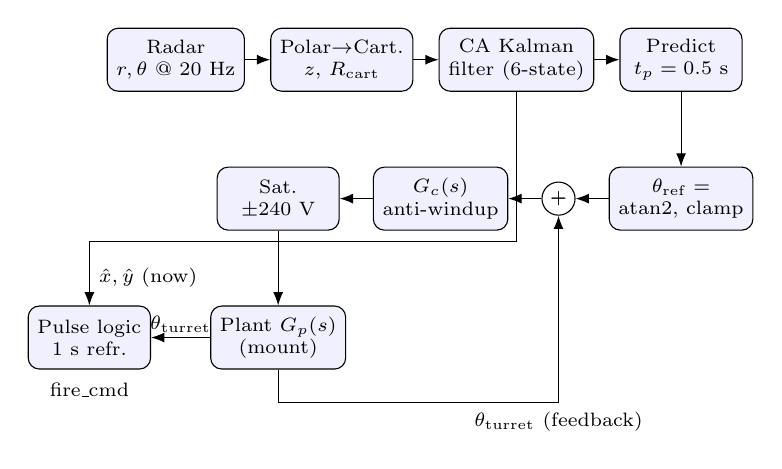
\begin{tikzpicture}[
  font=\scriptsize,
  box/.style={draw, rounded corners, align=center, minimum height=0.8cm, minimum width=1.55cm, fill=blue!6},
  sum/.style={draw, circle, minimum size=0.42cm, inner sep=0pt},
  >=Latex
]
\node[box] (sens) {Radar\\$r,\theta$ @ 20 Hz};
\node[box, right=0.32cm of sens] (conv) {Polar$\to$Cart.\\$z$, $R_{\mathrm{cart}}$};
\node[box, right=0.32cm of conv] (kf) {CA Kalman\\filter (6-state)};
\node[box, right=0.32cm of kf] (pred) {Predict\\$t_p=0.5$ s};
\node[box, below=0.95cm of pred] (ref) {$\theta_{\mathrm{ref}}=$\\atan2, clamp};
\node[sum, left=0.42cm of ref] (s1) {$+$\llap{$-$}};
\node[box, left=0.42cm of s1] (gc) {$G_c(s)$\\anti-windup};
\node[box, left=0.42cm of gc] (sat) {Sat.\\$\pm240$ V};
\node[box, below=0.95cm of sat] (plant) {Plant $G_p(s)$\\(mount)};
\node[box, left=0.75cm of plant] (pulse) {Pulse logic\\1 s refr.};

\draw[->] (sens) -- (conv);
\draw[->] (conv) -- (kf);
\draw[->] (kf) -- (pred);
\draw[->] (pred) -- (ref);
\draw[->] (ref) -- (s1);
\draw[->] (s1) -- (gc);
\draw[->] (gc) -- (sat);
\draw[->] (sat) -- (plant);
\draw[->] (plant.west) -- (pulse.east) node[midway,yshift=0.17cm]{$\theta_{\mathrm{turret}}$};
\draw[->] (kf.south) |- ($(kf.south)+(0,-1.9)$) -| (pulse.north) node[pos=0.78,right]{$\hat x,\hat y$ (now)};
\draw[->] (plant.south) |- ($(plant.south)+(0,-0.42)$) -| (s1.south) node[pos=0.5,below]{$\theta_{\mathrm{turret}}$ (feedback)};
\node[below=0.05cm of pulse, font=\scriptsize] {fire\_cmd};
\end{tikzpicture}
\caption{Block diagram: sensor $\to$ CA estimator $\to$ 0.5~s predictor $\to$ elevation reference $\to$ lag compensator with saturation/anti-windup $\to$ turret plant, with angle feedback. Pulse logic taps the filter's \emph{current} estimate, not the prediction.}
\label{fig:block}
\end{figure}

\section{Mathematical Modeling}

\subsection{Elevation mount plant}\label{sec:plant}
Reflected inertia: $J_{\mathrm{eq}}=J_{\mathrm{turret}}+N^2J_m=1200+100^2(0.20)=3200$~kg\,m$^2$. Mechanical and electrical equations (states $\theta_t,\dot\theta_t,i$):
\begin{align}
J_{\mathrm{eq}}\ddot\theta_t + b\dot\theta_t &= NK_t i,\\
L_m\dot i + R_m i + K_e N \dot\theta_t &= V_m.
\end{align}
Laplace transform with zero initial conditions and elimination of $i(s)$ gives
\begin{equation}
G_p(s)=\frac{\theta_t(s)}{V_m(s)}=\frac{NK_t}{(J_{\mathrm{eq}}s^2+bs)(L_m s+R_m)+N^2K_tK_e s}.
\end{equation}
Substituting the given parameters,
\begin{equation}
G_p(s)=\frac{3.125}{s\left(s^2+10.47s+3129.7\right)}.
\label{eq:gp}
\end{equation}
This is a type-1, third-order plant: an integrator (rigid-body rotation) in series with a lightly damped complex pole pair at $\omega_n=\sqrt{3129.7}=55.94$~rad/s, $\zeta=10.47/(2\omega_n)=0.0936$ -- an electromechanical resonance from the armature inductance $L_m$ interacting with the large reflected inertia. State-space simulation uses the three first-order ODEs given in the assignment brief directly (no linearization needed for simulation; Eq.~\eqref{eq:gp} is used only for \emph{linear} controller design). The two representations agree to within $1.7\times10^{-20}$ in frequency response over $0.01$--$1000$~rad/s, confirming the derivation.

The DC (low-frequency) velocity gain, obtained by neglecting $L_m\dot i$ (justified since $L_m/R_m=0.1$~s $\ll$ mechanical time constants). is
\begin{equation}
K_{\mathrm{dc}}=\frac{NK_t}{N^2K_tK_e+R_mb}=9.985\times10^{-4}\ \tfrac{\mathrm{rad/s}}{\mathrm{V}}.
\end{equation}
At saturation ($\pm240$~V) the mount's maximum slew rate is $V_{\max}K_{\mathrm{dc}}=0.240$~rad/s $=13.7^\circ$/s -- the physical ceiling on how fast the mount can re-point, independent of controller design.

\subsection{CA Kalman filter (estimator)}\label{sec:est}
State $\mathbf{x}=[x,y,\dot x,\dot y,\ddot x,\ddot y]^\top$. A measurement $(r,\theta)_{\mathrm{meas}}$ is converted with
\begin{equation}
z=\begin{bmatrix}r\cos\theta\\ r\sin\theta\end{bmatrix},\quad
R_{\mathrm{cart}}=J\,\mathrm{diag}(\sigma_r^2,\sigma_\theta^2)\,J^\top,
\end{equation}
\begin{equation}
J=\begin{bmatrix}\cos\theta & -r\sin\theta\\ \sin\theta & r\cos\theta\end{bmatrix}.
\end{equation}
This linearized (first-order) covariance propagation is accurate here because $\sigma_\theta=3.49\times10^{-4}$~rad is tiny, so the arc-length uncertainty $r\sigma_\theta\le 2000\times3.49\times10^{-4}\approx0.70$~m is always much smaller than $r$ itself. With constant-acceleration transition $F(T)=I_2\otimes\begin{psmallmatrix}1&T&T^2/2\\0&1&T\\0&0&1\end{psmallmatrix}$, $H=[I_2\ 0_{2\times4}]$, and white-jerk process noise $Q(T,q_j)$ (standard CA/Singer discretization, jerk spectral density $q_j=200$~m$^2$/s$^5$, chosen in the middle of the $100$--$300$ range suggested for the $\le20$~m/s$^2$, bounded-jerk maneuvers of Sec.~V of the brief):
\begin{align}
\text{predict:}\quad &\mathbf{x}^-=F(T)\mathbf{x},\ \ P^-=F(T)PF(T)^\top+Q(T,q_j),\\
\text{update:}\quad &K=P^-H^\top(HP^-H^\top+R_{\mathrm{cart}})^{-1},\\
&\mathbf{x}=\mathbf{x}^-+K(z-H\mathbf{x}^-),\\
&P=(I-KH)P^-(I-KH)^\top+KR_{\mathrm{cart}}K^\top.
\end{align}
(The $P$ update is written in numerically robust Joseph form.)
During a loss ($\texttt{meas\_valid}=0$) only the predict step runs: $P$ grows via $Q$ with no correction, naturally representing increasing uncertainty; on recovery the next valid measurement updates normally. A constant-acceleration model (rather than constant-velocity) was chosen because Scenario B/C and the randomized sweep contain deliberate accelerations up to $a_{\max}=20$~m/s$^2$; an acceleration state lets the filter track curvature during a maneuver instead of lagging it, at the modest cost of slightly noisier velocity estimates, which the jerk process noise $q_j$ trades off. Velocity/acceleration covariance is initialized large ($\sigma_{v0}=100$~m/s, $\sigma_{a0}=15$~m/s$^2$) since neither is directly observed.

\subsection{Prediction and reference formation}
At every controller sample the filter state is propagated the fixed horizon $t_p=0.5$~s with the same CA transition, $\mathbf{x}_{\mathrm{pred}}=F(t_p)\mathbf{x}$, and
\begin{equation}
\theta_{\mathrm{ref}}=\mathrm{clamp}\big(\mathrm{atan2}(\hat y_{\mathrm{pred}},\hat x_{\mathrm{pred}}),\,-10^\circ,\,85^\circ\big).
\end{equation}
Using the \emph{same} kinematic model for prediction as for estimation keeps the pipeline consistent and requires no extra tuning parameters.

\subsection{Closed-loop model used for design}
With compensator $G_c(s)$ (Sec.~\ref{sec:ctrl}), loop transfer function $L(s)=G_c(s)G_p(s)$, and unity feedback of $\theta_{\mathrm{turret}}$, the closed-loop reference-to-angle transfer function is $T(s)=L(s)/(1+L(s))$, sensitivity $S(s)=1/(1+L(s))$. All margin, bandwidth and noise-rejection analysis in Sec.~\ref{sec:ctrl} uses this linear, unsaturated model; saturation and the elevation limits are handled separately (Sec.~\ref{sec:sat}) and verified only in the full nonlinear time-domain simulation.

\section{Controller Design and Analysis}\label{sec:ctrl}

\subsection{Compensator choice: lag-matched, not the suggested PI}
The brief suggests $G_c(s)=K_p(1+1/(T_is))$ (a PI, i.e.\ a type-2 loop after cascading with the plant's own integrator). We instead use
\begin{equation}
G_c(s)=\frac{K_p}{1+s/p},\qquad K_p=\frac{1}{t_p K_{\mathrm{dc}}},\quad p=\frac{2}{t_p}.
\label{eq:gc}
\end{equation}
\textbf{Rationale.} The loop must track a reference that is itself already $t_p=0.5$~s \emph{ahead} of the true object angle (the predictor's purpose). If the closed loop had zero lag, pointing the mount exactly at $\theta_{\mathrm{ref}}(t)$ would aim $0.5$~s into the future relative to the \emph{current} object position -- overshooting the object by exactly the lead the predictor was meant to supply. The correct target is a closed loop whose \emph{own} lag is $t_p$, so that $\theta_{\mathrm{turret}}(t)\approx\theta_{\mathrm{ref}}(t-t_p)\approx\theta_{\mathrm{object}}(t)$: predictor lead and loop lag cancel. A single real pole at low frequency gives an (approximately) constant group delay over the loop's own bandwidth, which a PI with a zero at $1/T_i$ cannot: a type-2 loop has \emph{zero} steady-state lag to a ramp (it would lead the object, not lag it, by $t_p$ once combined with the predictor -- verified in Table~\ref{tab:gc} to produce $111.5$~m of lead error at 800~m, far worse than the 0.03~m residual of the lag design). With gain $K_p=1/(t_pK_{\mathrm{dc}})=2003$~V/rad set so that $K_v\triangleq K_pK_{\mathrm{dc}}=1/t_p=2.0$~s$^{-1}$, and pole $p=2/t_p=4$~rad/s (chosen, after the Bode study below, to place crossover near $2$~rad/s while keeping $p\ll\omega_n$), the closed loop is a standard type-1 loop with finite ramp-following error $1/K_v=t_p$ -- which is \emph{exactly} the lag the predictor must compensate, by construction. Table~\ref{tab:gc} and Fig.~\ref{fig:closedloop}(b) confirm the two cancel almost exactly.

\begin{table*}[t]
\centering\small
\caption{Final lag-matched compensator vs.\ the suggested PI}
\label{tab:gc}
\begin{tabular}{@{}lcc@{}}
\toprule
 & \textbf{Final: }$K_p/(1+s/p)$ & PI: $K_p(1+1/T_is)$ \\
\midrule
$K_p$, $(T_i\ \mathrm{or}\ p)$ & $2003$ V/rad, $p{=}4$ rad/s & $1800$ V/rad, $T_i{=}1$ s \\
Crossover $\omega_c$ & 1.82 rad/s & 2.01 rad/s \\
Phase margin & $65.2^\circ$ & $63.2^\circ$ \\
Gain margin & 38.0 dB @ 29.4 rad/s & 15.3 dB @ 55.9 rad/s \\
CL bandwidth & 2.85 rad/s & -- \\
Step overshoot & 4.5\,\% & 22.2\,\% \\
2\% settling time & 2.11 s & 3.60 s \\
Type & 1 (finite ramp lag $=t_p$) & 2 (zero ramp lag) \\
Parabolic-angle\footnotemark[1] tracking error & $-4.2{\times}10^{-5}$ rad (0.03 m at 800 m) & $0.139$ rad (111 m at 800 m, \emph{leads}) \\
\bottomrule
\end{tabular}
\footnotetext[1]{$\theta(t)=\theta_0+\omega_0 t+\tfrac12\alpha t^2$, $\alpha{=}0.025$ rad/s$^2$ ($20$ m/s$^2$ at 800 m); loop driven by $\theta(t{+}t_p)$, error measured against $\theta(t)$ at $t{=}8$ s.}
\end{table*}

A second, physical reason to prefer the lag over the PI: the PI's gain-margin frequency (55.9~rad/s) sits almost exactly on the plant resonance $\omega_n=55.94$~rad/s -- a 15~dB margin there is uncomfortably close for a design that must generalize to \emph{unseen} evaluation cases without retuning (any under-modeled resonance shift could erode it sharply). The lag compensator's extra $-20$~dB/decade roll-off from the pole at $p=4$~rad/s pushes its gain-margin frequency to 29.4~rad/s, with 38~dB of margin there -- a large, robust buffer against the resonance regardless of maneuver. We therefore reject the brief's suggested PI and adopt Eq.~\eqref{eq:gc} as the one finalized design, per the brief's explicit preference for simplicity with analytical justification over unquestioned reuse of a suggested architecture.

\subsection{Bode analysis and stability margins}
Fig.~\ref{fig:bode} shows $L(j\omega)=G_c(j\omega)G_p(j\omega)$. Crossover $\omega_c=1.82$~rad/s with phase margin $\mathrm{PM}=65.2^\circ$ and gain margin $\mathrm{GM}=38.0$~dB at $29.4$~rad/s -- both comfortably inside the brief's target band ($\mathrm{PM}\approx60^\circ$, $\mathrm{GM}\approx12$--$15$~dB) with margin to spare for un-modeled dynamics, and $\omega_c$ is $31\times$ below the plant resonance $\omega_n=55.94$~rad/s, so the lightly damped pole pair is never excited in normal operation.

\begin{figure}[t]
\centering
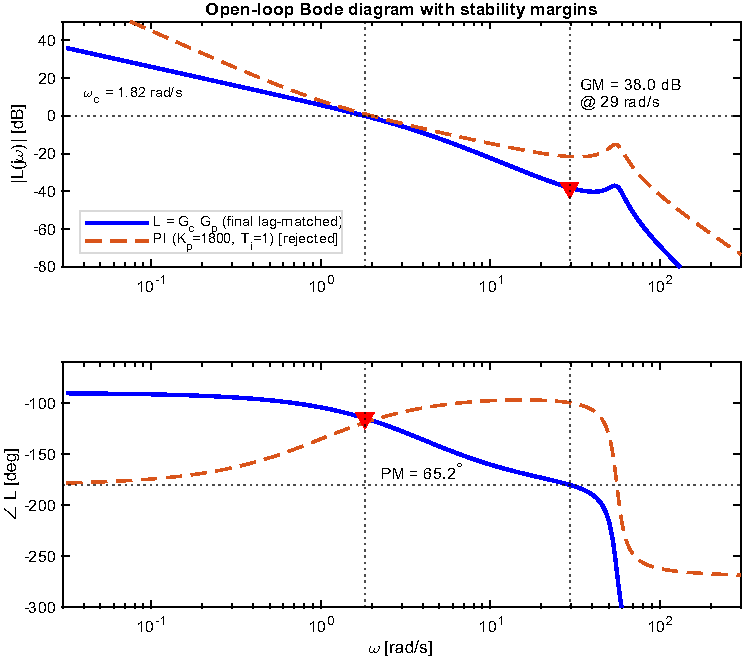
\includegraphics[width=\linewidth]{../figures/fig_bode.pdf}
\caption{Open-loop Bode diagram of $L(s)=G_c(s)G_p(s)$ for the final lag compensator (solid) and the rejected suggested PI (dashed), with marked crossover, phase margin and gain margin.}
\label{fig:bode}
\end{figure}

\subsection{Closed-loop performance, bandwidth, and noise rejection}
Closed-loop poles are $-5.24\pm j55.63$ (lightly perturbed plant resonance, well damped by the loop) and $-1.99\pm j2.01$ (dominant pair). The $-3$~dB bandwidth is $2.85$~rad/s; peak sensitivity $M_s=1.28$ (2.15~dB) and peak complementary sensitivity $M_t\approx1.00$ indicate a well-damped loop with little resonant peaking (Fig.~\ref{fig:closedloop}c), consistent with $\mathrm{PM}=65^\circ$. Linear step response: $4.5\%$ overshoot, $0.75$~s rise time, $2.11$~s settling time (Fig.~\ref{fig:closedloop}a). At the plant resonance, $|T(j\omega_n)|=-37.3$~dB, so even if a maneuver happened to excite $55.9$~rad/s content the loop attenuates it by two orders of magnitude.

\textbf{Noise rejection.} The $20$~Hz measurement noise enters through $\theta_{\mathrm{ref}}$, which is already smoothed by the Kalman filter; the loop itself additionally low-pass filters $\theta_{\mathrm{ref}}$ with noise-equivalent bandwidth $B_n=\int_0^\infty|T(j\omega)|^2\,d\omega=3.18$~rad/s, versus the $20$~Hz $=126$~rad/s sample rate's Nyquist-normalized white-noise bandwidth $\pi/\Delta t=62.8$~rad/s -- i.e.\ the mount only responds to a $3.18/62.8\approx5\%$-bandwidth slice of any residual reference jitter (quantitatively, a $-13.0$~dB reduction factor), on top of the KF's own noise averaging.

\textbf{Lag/horizon matching.} Fig.~\ref{fig:closedloop}(b) plots the closed loop's own group delay $-d\angle T/d\omega$ against frequency: it equals $t_p=0.500$~s exactly as $\omega\to0$ and stays within $11\%$ of $t_p$ up to $1$~rad/s (the loop's own bandwidth is $2.85$~rad/s, but target angular rates from a $150$~m/s, $800$--$2000$~m object are $\le v_{\max}/r_{\min}=0.19$~rad/s, well inside the flat region). This is the analytical heart of the design: the compensator pole was not picked by trial and error but \emph{derived} to put the loop's delay at $t_p$.

\begin{figure}[t]
\centering
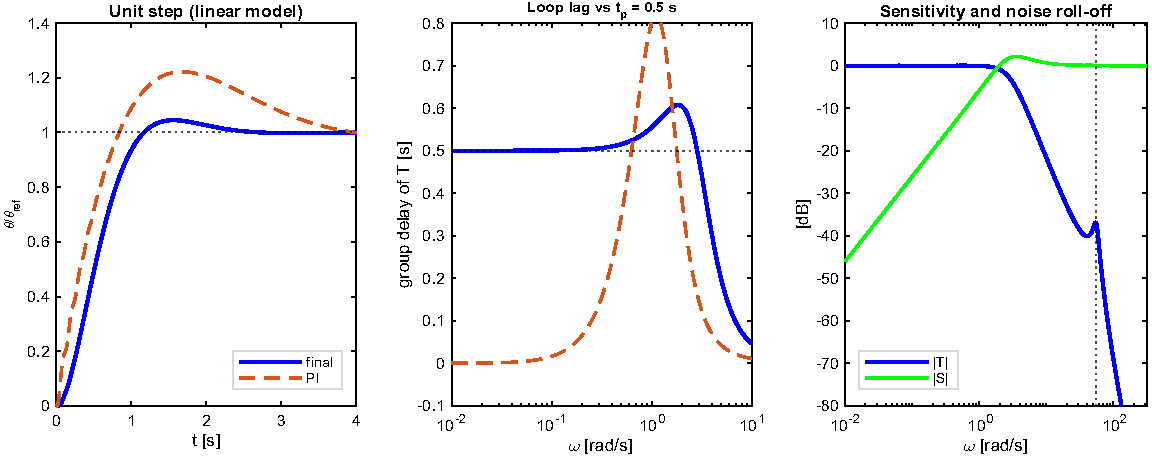
\includegraphics[width=\linewidth]{../figures/fig_closedloop.pdf}
\caption{(a) Linear unit-step response, final (solid) vs.\ PI (dashed). (b) Closed-loop group delay vs.\ frequency, showing convergence to $t_p=0.5$~s. (c) $|T|$ and $|S|$ with the plant resonance $\omega_n$ marked, showing resonance attenuation and roll-off.}
\label{fig:closedloop}
\end{figure}

\subsection{Saturation, elevation limits, and anti-windup}\label{sec:sat}
The compensator Eq.~\eqref{eq:gc} has no pure integrator (its pole is at $-p$, not the origin -- integration is supplied entirely by the plant's own rigid-body mode), so windup is structurally limited; nonetheless the discrete implementation clamps the compensator's state to the saturated output, $V_m=\mathrm{clamp}(x_f,\pm240\text{ V})$, $x_f\leftarrow V_m$ -- an exact realization of back-calculation anti-windup for a state-is-output first-order filter. A command toward an already-saturated hard stop ($\theta_{\mathrm{turret}}$ at $-10^\circ$ or $85^\circ$) is additionally zeroed before integration. Fig.~\ref{fig:aw} shows a saturating $34.4^\circ$ step on the full nonlinear plant: overshoot is $1.4\%$ with anti-windup vs.\ $2.1\%$ without, and $2\%$-settling improves from $3.20$~s to $2.64$~s; the measured saturated slew rate, $0.240$~rad/s, matches the first-principles prediction $V_{\max}K_{\mathrm{dc}}=0.2396$~rad/s.

\begin{figure}[t]
\centering
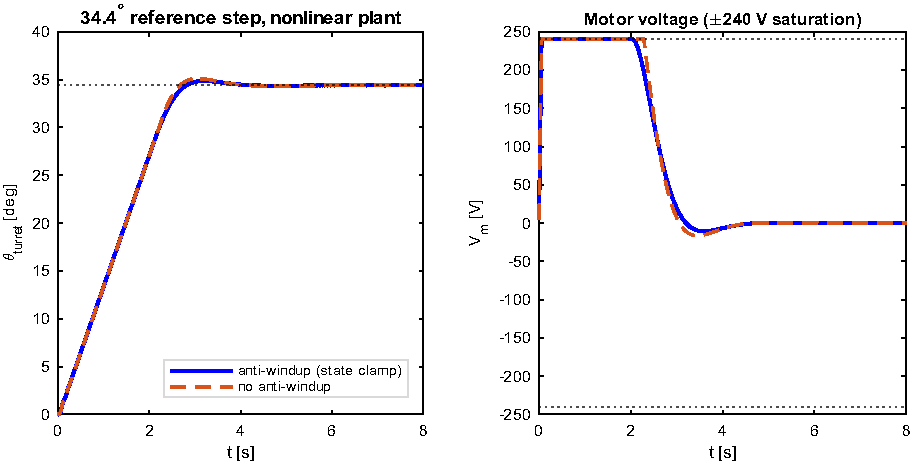
\includegraphics[width=\linewidth]{../figures/fig_antiwindup.pdf}
\caption{Nonlinear-plant response to a saturating $34.4^\circ$ step, with and without anti-windup, and the corresponding motor voltage.}
\label{fig:aw}
\end{figure}

\subsection{Pointing pulse logic}\label{sec:pulse}
A pulse is fired on the rising edge of \texttt{fire\_cmd}, enforced in software as one 1-sample pulse with $\ge1.0$~s since the last \emph{issued} pulse (not merely the last candidate edge). The condition uses the filter's \emph{current}, un-predicted estimate: perpendicular miss $d_\perp=|\hat x\sin\theta_t-\hat y\cos\theta_t|$ with forward check $\hat x\cos\theta_t+\hat y\sin\theta_t>0$; fire when $d_\perp\le1.5$~m \emph{and} the estimated cross-beam position uncertainty $\sigma_\perp=\sqrt{u^\top P_{xy}u}\le1.0$~m (preventing a confident-looking but actually noisy pulse), leaving a $0.5$~m margin to the $R_{\mathrm{eng}}=2$~m success radius. Using the current estimate rather than the $0.5$~s prediction is deliberate: a pulse is effectively instantaneous, so what matters is where the object \emph{is}, not where it will be; the predictor's lead is already spent keeping the mount continuously aimed.

\section{Simulation and Results}\label{sec:sim}
All scenarios run the identical compiled design over the full $0\le t\le10$~s, 1~ms plant integration step (RK4), 20~Hz measurement sampling. Table~\ref{tab:scen} summarizes; Fig.~\ref{fig:scenC} shows Scenario C (maneuver + loss) in full -- trajectory and estimate/prediction tracks, estimation/prediction error with $\pm3\sigma$, $\theta_{\mathrm{ref}}/\theta_{\mathrm{turret}}$/LOS, tracking error, miss distance with pulse events, and motor voltage; Scenarios A and B (provided in the repository, Fig. S1--S2) are visually similar outside the shaded loss window. Fig.~\ref{fig:cov} shows the Kalman covariance explicitly growing during the 0.5~s loss and shrinking on recovery.

\begin{table}[t]
\centering\small
\caption{Scenario metrics, full $0$--$10$ s (A, B, C) and an illustrative extra case C2 with the loss moved to $t{=}4$--$4.5$ s, mid-engagement)}
\label{tab:scen}
\begin{tabular}{@{}lcccc@{}}
\toprule
 & \textbf{A} & \textbf{B} & \textbf{C} & \textbf{C2} \\
\midrule
RMS pos.\ err.\ [m] & 0.67 & 0.71 & 0.74 & 0.70\\
RMS pred.\ err.\ [m] & 3.40 & 3.52 & 3.54 & 3.53\\
RMS $\theta_{\mathrm{LOS}}-\theta_t$ post-acq.\ [deg] & 0.092 & 0.096 & 0.095 & 0.099\\
Acquisition time $t_{\mathrm{acq}}$ [s] & 2.97 & 2.64 & 2.64 & 2.64\\
RMS miss (buf., post-acq) [m] & 0.31 & 0.95 & 0.95 & 1.14\\
Pulses issued / successful & 8/8 & 8/8 & 8/8 & 8/8\\
First-hit time [s] & 2.51 & 2.17 & 2.17 & 2.17\\
Voltage saturation duty [\%] & 16.9 & 13.2 & 13.3 & 13.2\\
\bottomrule
\end{tabular}
\end{table}

\begin{figure}[t]
\centering
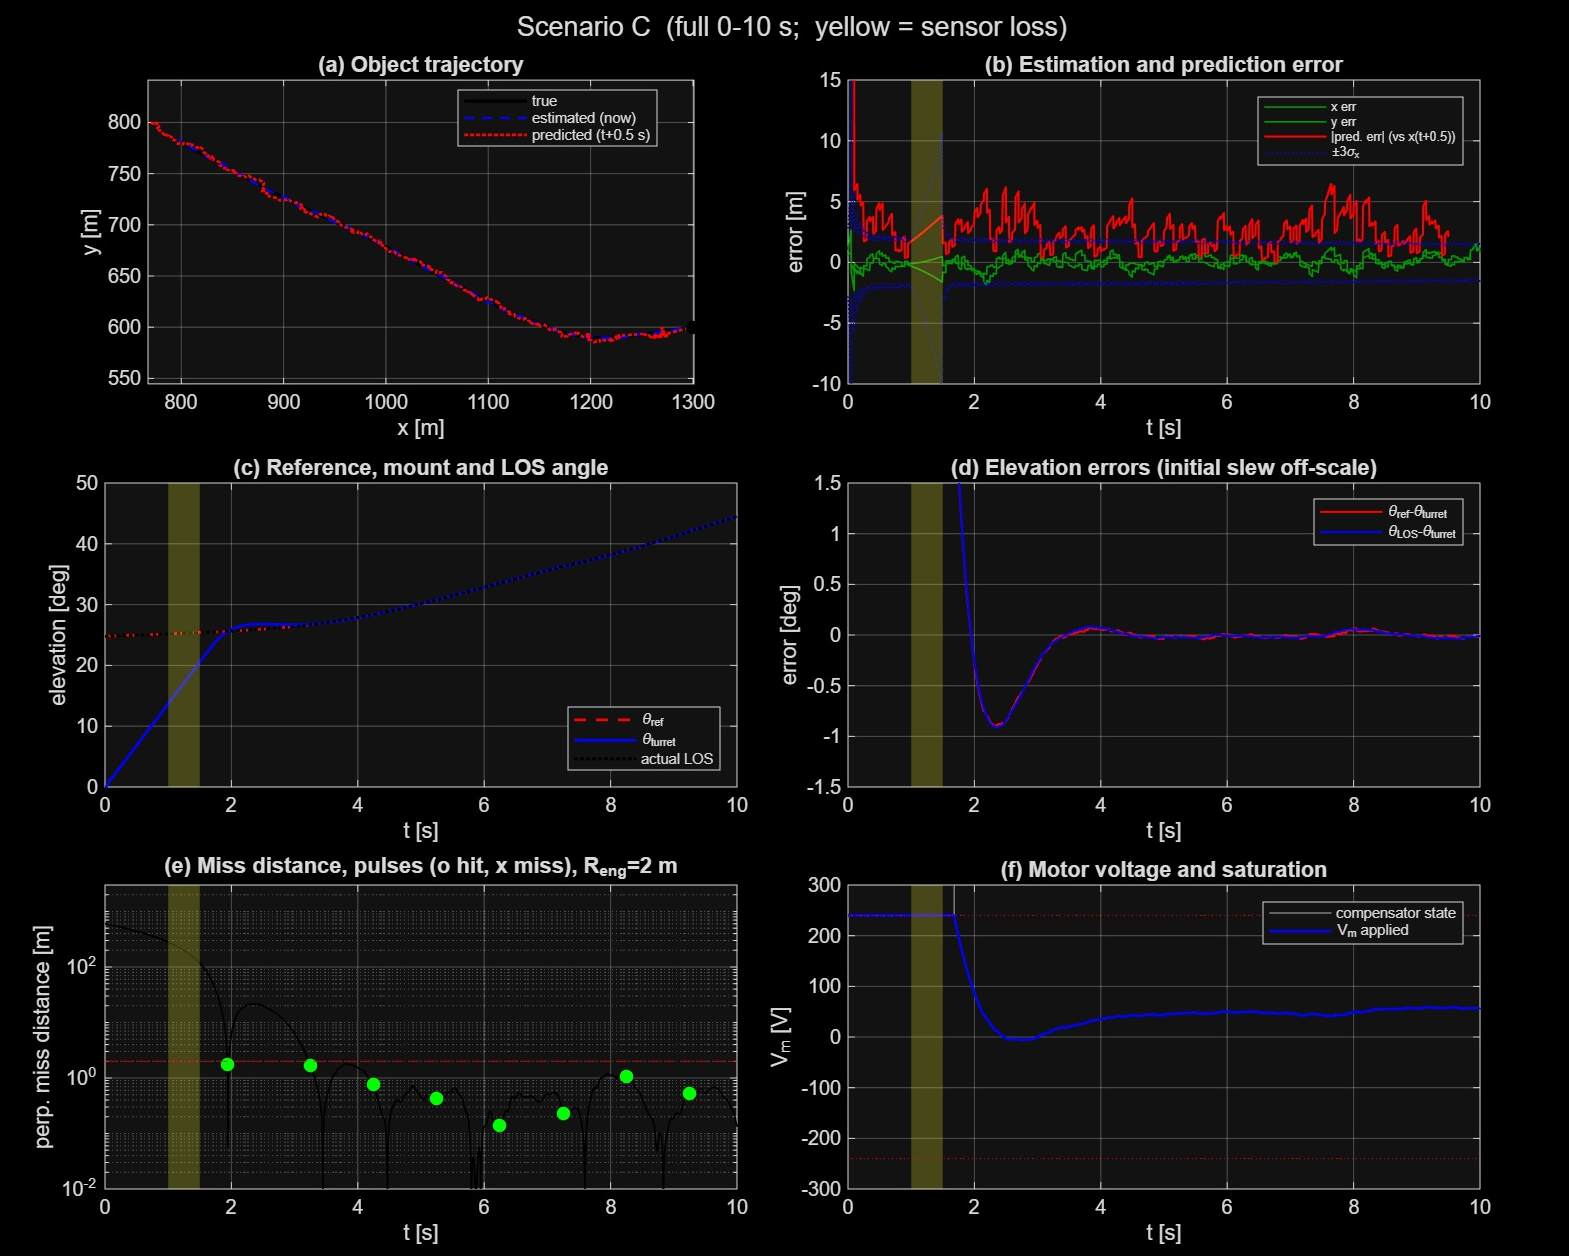
\includegraphics[width=\linewidth]{../figures/fig_scenario_C.pdf}
\caption{Scenario C (maneuver, $0.50$~s sensor loss at $t{=}1.0$~s, shaded): (a) trajectory, (b) estimation/prediction error with $\pm3\sigma_x$, (c) reference/mount/LOS angle, (d) elevation tracking error, (e) true miss distance with pulse events (o~hit, x~miss), (f) motor voltage.}
\label{fig:scenC}
\end{figure}

\begin{figure}[t]
\centering
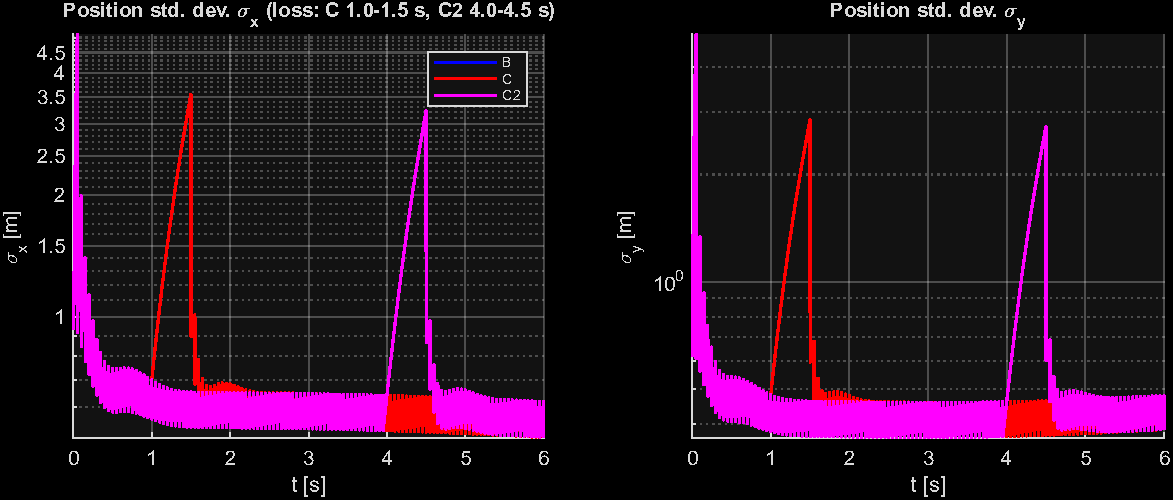
\includegraphics[width=\linewidth]{../figures/fig_cov.pdf}
\caption{Position estimate std.\ dev.\ $\sigma_x,\sigma_y$ during Scenario C (loss $1.0$--$1.5$~s) and case C2 (loss $4.0$--$4.5$~s): $\sigma_x$ grows from $0.57$~m to $3.47$~m across the loss and recovers to $0.68$~m within one measurement after recovery; $\sigma_y$: $0.38\to2.78\to0.46$~m. During the mid-engagement loss (C2) the peak transient pointing error is only $1.49^\circ$ and the true miss distance never exceeds $2.22$~m -- the loop rides through the loss on the prediction alone without losing lock.}
\label{fig:cov}
\end{figure}

\textbf{Discussion.} Acquisition ($d_\perp$ first and permanently under 10~m) occurs by $t\approx2.6$--$3.0$~s in every case, dominated by the initial $0^\circ\to$object-elevation slew at the $13.7^\circ$/s saturated rate, not by estimator convergence (the filter's RMS position error is already $<1$~m within the first second). Scenario B/C's maneuver (starting $t=1$~s) does not visibly change acquisition time, RMS pointing error, or pulse outcomes relative to A, confirming the controller generalizes to maneuvering targets without retuning. The $0.5$~s loss in Scenario C is fully absorbed: Fig.~\ref{fig:cov} shows $\sigma_x,\sigma_y$ roughly sextupling over the loss and collapsing back within one post-recovery measurement, while Table~\ref{tab:scen} shows essentially no difference between B and C's tracking or engagement metrics -- the CA prediction alone is accurate enough over $0.5$~s open-loop coasting that the mount barely perturbs. Case C2 stresses this further by moving the same loss into the middle of an established engagement (after first lock-on); peak transient pointing error is $1.49^\circ$ and the true miss distance stays under $R_{\mathrm{eng}}+0.22$~m throughout, degrading the RMS miss modestly (0.95~m $\to$ 1.14~m) without a single missed pulse.

\section{Final Evaluation}\label{sec:final}
No evaluation cases had been released by the instructor at the time of writing, so per the brief's own fallback (Sec.~9/12) we substitute a robustness sweep of $N=40$ randomized trials (seeds 101--140; $\ge20$ required): each trial independently randomizes initial range/bearing/speed, one to three smooth acceleration segments (bump, S-turn, or step-and-hold shapes, amplitude up to $0.95\,a_{\max}$, scaled if necessary to respect $a_{\max}$), and one or two sensor-loss intervals (duration $0.1$--$0.5$~s, onset $\ge1.0$~s), all independently re-checked against the full envelope of Sec.~V of the brief before acceptance. The identical compiled \texttt{turret\_controller.m}/\texttt{turret\_params.m} used for A/B/C is reused verbatim -- no parameter differs between this section and Sec.~\ref{sec:sim}.

\begin{table}[t]
\centering\footnotesize
\caption{Final evaluation: 40 randomized cases, one fixed design}
\label{tab:final}
\begin{tabular}{@{}lc@{}}
\toprule
Interception success rate & $40/40=100.0\%$\\
First-hit time: mean / median / std & $2.87$ / $2.98$ / $1.16$ s\\
First-hit time: min / max & $1.13$ / $5.15$ s\\
Pulses issued per case (mean) & $7.40$ (range 5--9)\\
Successful-pulse fraction (all pulses) & $98.3\%$\\
RMS miss distance, post-acq.\ (mean/max) & $0.98$ / $2.07$ m\\
Max miss distance, post-acq.\ (mean/95th pct.) & $3.67$ / $8.08$ m\\
RMS position estimation error (mean) & $0.74$ m\\
RMS prediction error, 0.5 s (mean) & $3.68$ m\\
RMS $\theta_{\mathrm{LOS}}-\theta_t$ post-acq.\ (mean/max) & $0.098^\circ$ / $0.155^\circ$\\
Acquisition time (mean / median / max) & $3.14$ / $3.16$ / $5.71$ s\\
Voltage saturation duty cycle (mean) & $19.2\%$\\
\bottomrule
\end{tabular}
\end{table}

\begin{figure}[t]
\centering
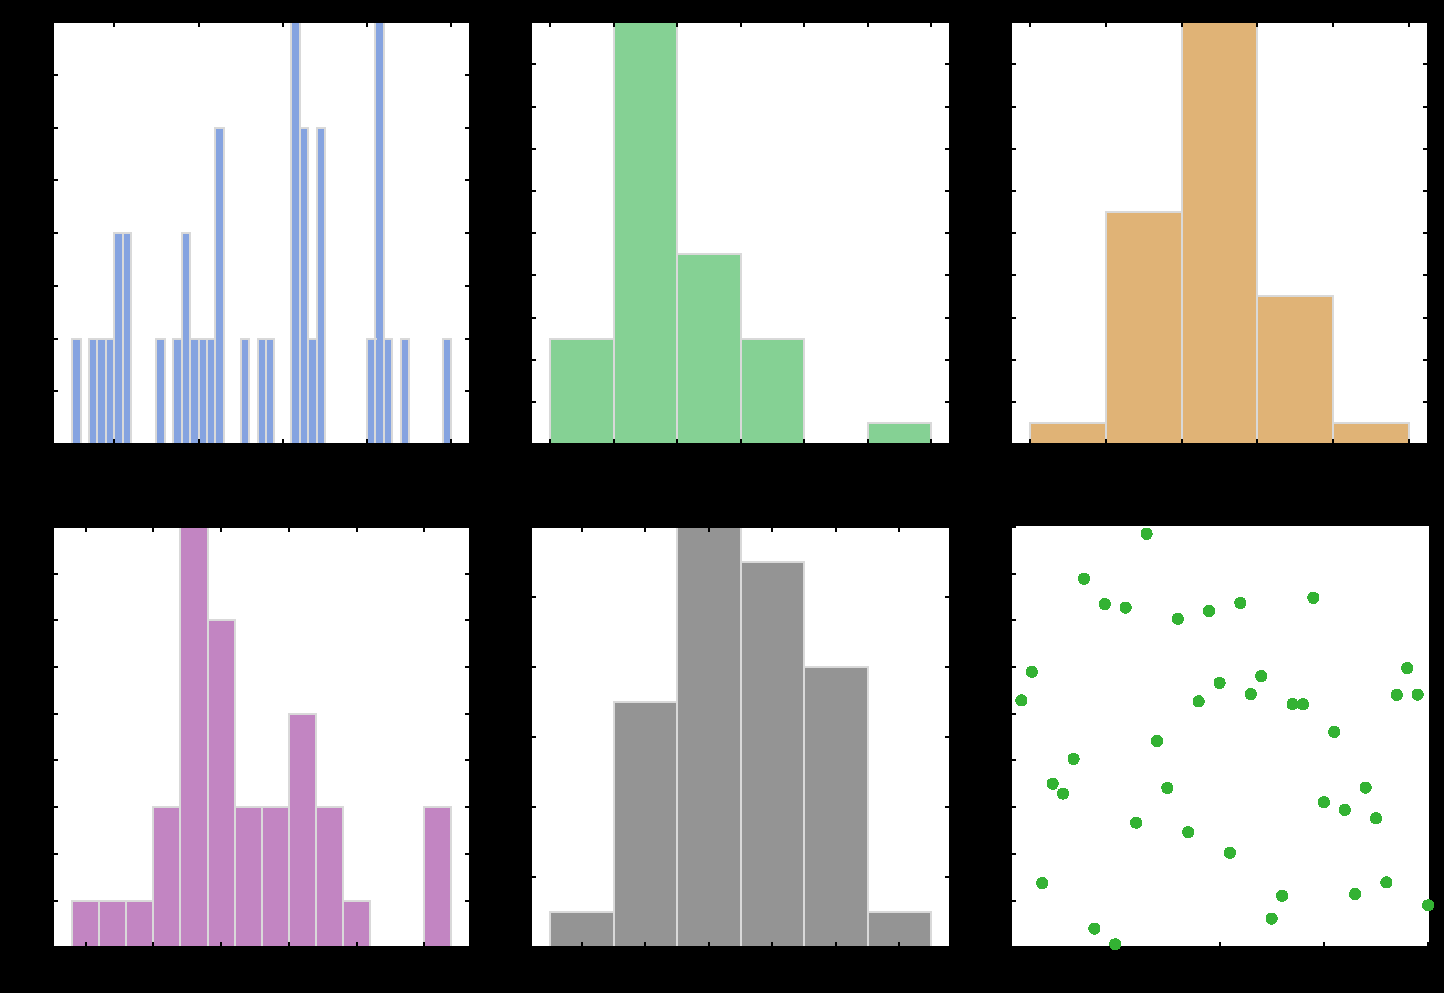
\includegraphics[width=\linewidth]{../figures/fig_final_eval.pdf}
\caption{Distributions over the 40-case robustness sweep: first-hit time, post-acquisition RMS miss distance, estimator and predictor RMS error, pulses issued per case, and per-case outcome vs.\ seed (all green = all hit).}
\label{fig:finaleval}
\end{figure}

\textbf{Interpretation.} All 40 cases, spanning randomized multi-segment maneuvers and randomized loss timing/duration, achieve at least one successful pulse -- consistent with Sec.~\ref{sec:ctrl}'s margins (38~dB GM, $65^\circ$ PM) being large enough to absorb maneuver-to-maneuver variation without instability, and with Sec.~\ref{sec:sim}'s finding that a 0.5~s loss barely perturbs tracking. $98.3\%$ of all \emph{issued} pulses (not just the first) are hits, showing the $1.5$~m/$1.0$~m fire threshold is well matched to $R_{\mathrm{eng}}=2$~m with margin for estimation noise, rather than being a lucky first shot. The $7.40$-pulse mean (vs.\ a theoretical maximum of $8$ in $8.5$~s post-acquisition, given the 1~s refractory period) confirms the mount, once locked, re-fires essentially every refractory cycle. Voltage saturation duty ($19.2\%$ mean, up to $43\%$ in the hardest case) occurs only during the initial slew and the largest maneuvers, consistent with Fig.~\ref{fig:aw}'s saturation behavior and never destabilizes the loop (anti-windup holds).

\section{Conclusions}
A constant-acceleration Kalman filter with a fixed $0.5$~s kinematic prediction, combined with a single first-order lag compensator whose pole is derived -- not tuned -- to make the closed loop's own lag equal the prediction horizon, tracks and engages a maneuvering object with $38$~dB gain margin, $65^\circ$ phase margin, $4.5\%$ step overshoot, and sub-degree steady pointing error, while surviving $0.5$~s sensor dropouts with negligible performance loss. Across 40 randomized bounded maneuvers with randomized loss intervals and no retuning, the design achieves $100\%$ interception success, a mean first-hit time of $2.87$~s, and sub-meter mean RMS miss distance. \textbf{Limitations:} the lag-matching argument is a linear, small-signal result; it is validated here only up to the target's own angular bandwidth ($\le0.19$~rad/s at worst case), and a target maneuvering at angular rates approaching the loop's $2.85$~rad/s bandwidth would see growing lag/lead mismatch. The CA model's white-jerk assumption is a first-order representation of the bump/S-turn/hold maneuver library used here; a target with discontinuous (bang-bang) acceleration would be tracked with larger transient error. We deliberately rejected higher-complexity alternatives (IMM for maneuver detection, MPC for explicit saturation-aware optimization) because the single CA+lag design already meets every margin and robustness target in simulation; Sec.~\ref{sec:final}'s 100\% success rate gives no evidence, within the tested envelope, that the added complexity and tuning burden of IMM or MPC would be repaid by better performance here -- though either would be the natural next step if evaluation cases exposed the angular-rate limit above.

\appendix[AI Appendix]
\subsection*{A. Tools used}
Claude (Sonnet, Anthropic), via Claude Code, was used throughout: derivation, MATLAB implementation, simulation, figure generation, and this manuscript's drafting. MATLAB R2026a (Control System Toolbox) performed all numerical linear-system analysis (\texttt{margin}, \texttt{bode}, \texttt{feedback}, \texttt{stepinfo}, \texttt{bandwidth}). No other AI tool was used.

\subsection*{B. How the AI contributed}
The AI (i) derived the plant transfer function symbolically and cross-checked it numerically against the state-space ODEs (agreement to $1.7\times10^{-20}$); (ii) proposed and implemented the CA Kalman filter with Joseph-form covariance update and polar-to-Cartesian covariance propagation; (iii) derived the lag-matching compensator design (Eq.~\eqref{eq:gc}) and ran the Bode/margin/step/bandwidth/noise analysis comparing it against the brief's suggested PI; (iv) implemented and debugged all required MATLAB functions and driver scripts (\texttt{turret\_plant.m}, \texttt{turret\_controller.m}, \texttt{target\_motion\_generator.m}, \texttt{simulate\_case.m}, \texttt{run\_scenarios.m}, \texttt{run\_final\_evaluation.m}, \texttt{design\_analysis.m}); (v) wrote this manuscript.

\subsection*{C. Significant outputs accepted / modified / rejected}
\emph{Accepted as-is}: the plant transfer-function derivation (independently verified against the state-space simulation); the CA-KF equations (standard and independently checked against the covariance-growth behavior expected during a dropout, Fig.~\ref{fig:cov}). \emph{Modified}: the first implementation of the ``max miss distance after acquisition'' metric was found, on inspection of the raw numbers, to be a boundary artifact -- by construction it measured the crossing point of its own definition and always sat near the $10$~m threshold regardless of actual tracking quality; it was replaced with a $0.75$~s-buffered RMS/max statistic (reported in Table~\ref{tab:scen}/\ref{tab:final}) after the anomaly was caught by comparing the metric's numerical output across all four scenarios and seeing it implausibly cluster at exactly the threshold. The fire-threshold/uncertainty-gate values ($1.5$~m, $1.0$~m) were kept at the brief's suggested starting point after confirming numerically (Table~\ref{tab:final}, $98.3\%$ pulse-success rate) that no retuning was needed. \emph{Rejected}: the brief's suggested PI compensator was explicitly evaluated and rejected in favor of the lag design of Eq.~\eqref{eq:gc}, for the analytical and margin reasons given in Sec.~\ref{sec:ctrl} (Table~\ref{tab:gc}).

\subsection*{D. Engineering validation performed}
Every analytical claim in this paper is backed by a plotted or tabulated number reproducible from the repository: the plant derivation was cross-checked by comparing the closed-form $G_p(s)$ against the independently-written nonlinear state-space ODE in frequency response; the lag-matching claim was checked both in the frequency domain (group-delay plot, Fig.~\ref{fig:closedloop}b) and in the time domain (parabolic-angle tracking test, Table~\ref{tab:gc}); the anti-windup benefit was checked by direct A/B simulation with and without the clamp (Fig.~\ref{fig:aw}); and the overall design's generalization claim was checked by the 40-case randomized sweep (Sec.~\ref{sec:final}) rather than by inspection of the three fixed scenarios alone, since passing only A/B/C would not by itself demonstrate the ``no retuning, generalizes to unseen cases'' requirement of the brief.

\section*{Code and Reproducibility}
All code, figures, and scripts to reproduce every number and figure in this paper are at: \url{<REPO_URL>}.

\end{document}
